\documentclass{beamer}

\author[Team PattReco5]{}
\institute{\bf A PRESENTATION TOPIC BELONGS TO LATEX }
\title{\bf \underline{PATTERN RECOGNITION}}

\usepackage{multimedia}
\usepackage{animate}
\usepackage{color}
\usepackage{hyperref}
\usepackage{xcolor}
\usepackage{amssymb}
%\titlegraphic{\includegraphics[width=2cm]{mlnc.png}%\hspace*{}~%
   
%}
%\institute{\bf Motilal Nehru College Of Delhi University}
%%%%%%%%%%%%%%%%%%%%%%%%%%%%%%%%%%%%%%%


\usepackage{tikz}
\usepackage{verbatim}

\usetikzlibrary{calc,trees,positioning,arrows,chains,shapes.geometric,%
    decorations.pathreplacing,decorations.pathmorphing,shapes,%
    matrix,shapes.symbols}

\tikzset{
>=stealth',
  punktchain/.style={
    rectangle, 
    rounded corners, 
    % fill=black!10,
    draw=black, very thick,
    text width=8em, 
    minimum height=1.5em, 
    text centered, 
    on chain},
  line/.style={draw, thick, <-},
  element/.style={
    tape,
    top color=white,
    bottom color=blue!50!black!60!,
    minimum width=5em,
    draw=blue!40!black!90, very thick,
    text width=5em, 
    minimum height=1.5em, 
    text centered, 
    on chain},
  every join/.style={->, thick,shorten >=.5pt},
  decoration={brace},
  tuborg/.style={decorate},
  tubnode/.style={midway, right=1pt},
}








%%%%%%%%%%%%%%%%%%%%%%%%%%%%%%%%%%%%%%%%%%%%%%%

\usetheme{Warsaw}
%\usetheme{Singapore}
%\definecolor{unitednationsblue}{rgb}{0.36, 0.57, 0.9}
\definecolor{mygreen}{rgb}{0.125,0.5,0.25}
%\usecolortheme{fly}
\usecolortheme[named=mygreen]{structure}
\usepackage{graphicx}
\usepackage{enumerate}
%\renewcommand{\lableitem}{$\ast$}
\date{\bf{October 27, 2018}}

 \setbeamertemplate{background}{\tikz[overlay,remember picture]\node[opacity=0.4]at (current page.center){\includegraphics[width=\paperwidth]{thmb.jpg}};}%this command is use to add water mark in hole                 %%%%%%%%%%%%%%%%%%%%%%%%%%%%%%%%%%%%%%%%%%%%%%%%%%%%%%presentation.


\usepackage{tikz}%this package is also help to add water mark.
\usepackage{kantlipsum}%this package is also help to add water mark.


\expandafter\def\expandafter\insertshorttitle\expandafter{%this command is use for page no. in beamer.
  \insertshorttitle\hfill%%this command is use for page no. in beamer.
  \insertframenumber\,/\,\inserttotalframenumber}%this command is use for page no. in beamer.

\begin{document}
\begin{frame}
\transwipe

\begin{columns}


\begin{column}{.35\textwidth}
\hspace{1.cm}
\includegraphics[width=.35\textwidth]{mlnc.png}%{\hspace{1.5cm}} \pause
\end{column}


\begin{column}{.6\textwidth}
{\bf \underline{MOTILAL NEHRU COLLEGE }}\\ \hspace{.4cm}{\bf \underline{ UNIVERSITY OF DELHI }}
\end{column}


\begin{column}{.4\textwidth}
\includegraphics[width=.4\textwidth]{du.jpg}%{\hspace{1cm}} %\pause
\end{column}


\end{columns}
\hspace{2.2cm} {\bf \underline{DEPARTMENT OF MATHEMATICS }}\\


\titlepage


\end{frame}

\begin{frame}
%\transpush

\frametitle{GROUP MEMBERS DETAILS} \pause
\begin{enumerate}

\begin{columns}
\begin{column}{.5\textwidth}
\item[$\triangleright$] HARIOM
\end{column}


\begin{column}{.5\textwidth}
\item[$\unrhd$] MTH17097
\end{column}
\end{columns}
\pause

\begin{columns}
\begin{column}{.5\textwidth}
\item[$\triangleright$]ANSHUL 
\end{column}


\begin{column}{.5\textwidth}
\item[$\unrhd$] MTH17095
\end{column}
\end{columns}
\pause

\begin{columns}
\begin{column}{.5\textwidth}
\item[$\triangleright$]POOJA AHUJA
\end{column}


\begin{column}{.5\textwidth}
\item[$\unrhd$] MTH17092
\end{column}
\end{columns}
\pause

\begin{columns}
\begin{column}{.5\textwidth}
\item[$\triangleright$]GOVIND SHAHU
\end{column}


\begin{column}{.5\textwidth}
\item[$\unrhd$] MTH17094
\end{column}
\end{columns}
\pause
\begin{columns}
\begin{column}{.5\textwidth}
\item[$\triangleright$]MUNNA KUMAR YADAV
\end{column}


\begin{column}{.5\textwidth}
\item[$\unrhd$] MTH17091
\end{column}
\end{columns}
\pause

\end{enumerate}
\end{frame}

\begin{frame}
%\transpush
\transblindshorizontal
%\begin{center}
\frametitle {CONTENTS} %\pause
%\end{center}
\begin{itemize}
\begin{columns}
\begin{column}{.5\textwidth}
\item \onslide<2->INTRODUCTION %\pause
\item \onslide<3-> PATTERN% \pause
\item \onslide<4-> PATTERN RECOGNITION %\pause
\end{column}
\onslide<1->
\begin{column}{.2\textwidth}
\includegraphics[width=\textwidth]{cont.png}


\end{column}
\end{columns}
\item \onslide<5-> PATTERN RECOGNITION SYSTEM %\pause
\item \onslide<6-> PATTERN RECOGNITION MODEL %\pause
\item \onslide<7-> APPLICATION OF PATTERN RECOGNITION% \pause

\item \onslide<8-> CASE STUDY %\pause
\item \onslide<9-> ADVANTAGE AND DISADVANTAGE% \pause
\item \onslide<10-> CONCLUSION %\pause
\item \onslide<11-> FUTURE WORK %\pause
\item \onslide<12> REFERENCES %\pause

\end{itemize}
\end{frame}

\begin{frame}
\transboxout
\frametitle{INTRODUCTION} 

\begin{itemize}
\begin{columns}
\begin{column}{.5\textwidth}
\item [$\ast$] \onslide<2-> Pattern Recognition is a branch of Artificial Intelligence. 

\item[$\ast$]\onslide<3-> Humans can recognize the faces without worrying about the varying illuminations. When implementing such recognition artificially, it becomes a very complex task. 


\item[$\ast$] \onslide<4>The field of Artificial Intelligence has made this complex task possible. 

\end{column}
\onslide<1->
\begin{column}{.5\textwidth}
\includegraphics[width=\textwidth]{intro.jpg}
\end{column}
\end{columns}
\end{itemize}



\end{frame}

\begin{frame}
\transblindsvertical
\frametitle{PATTERN}
\begin{itemize}
\item \onslide<2-> A Pattern is a set of objects or phenomena or concepts where the element of the set are similar to one another in certain ways or aspects. %\pause
\item \onslide<3-> A Pattern is an entity, that could be given a name.  %\pause
\begin{itemize}
\vspace{1cm}\item[Example:-]\onslide<4-> 
\end{itemize}
\end{itemize}
\begin{columns}
\onslide<5->
\begin{column}{.3\textwidth}
\begin{figure}
\includegraphics[width=\textwidth]{finger.jpg} 
\caption {Fingerprint}
\end{figure}
%\pause

\end{column}
\onslide<6->
\begin{column}{.3\textwidth}
\begin{figure}
\includegraphics[width=\textwidth]{hand.jpg}
\caption {Handwitten}
\end{figure}
\end{column}
%\pause

\begin{column}{.3\textwidth}
\onslide<7>
\begin{figure}
\includegraphics[width=\textwidth]{dna.jpg}
\caption {DNAsequence}
\end{figure}

\end{column}
\end{columns}

 
\end{frame}

\begin{frame}
\transdissolve

\frametitle{PATTERN RECOGNITION}%\pause
\begin{itemize}
\item \onslide<2->
 Pattern recognition is the procedure of processing and analizing diverse information(numerical,literal,logical) characterizing the objects or phenomenon, so as to provide descriptions, identification, classification and interpreations for them.
 \item \onslide<3-> {{\bf{``\underline {Perceive + Process +Prediction}" :-}} It is the study of how machine can}
 \begin{itemize}
 \item[$\diamond$] \onslide<4->
Perceive: Observe the environment(i.e. Interact with the real-world). 
 \item[$\diamond$]\onslide<5->
Process: Learn to distinguish pattern of interest from their background. 
 \item[$\diamond$]\onslide<6>
 Prediction: Make sound and reasonable decisions about the categories of the pattern. 
 \end{itemize}
\end{itemize}
\end{frame}


\begin{frame}
\transboxout

\frametitle{Evolution of Pattern Recognition}

\hspace{2cm}Looking at the history,pattern recognition system has come a long way.Earlier it was confined to theoretical research in the field of statistics for deriving various models out of the large amount of data.With the advent in computer technology,number of practical applications is increased in manifold which lead to further theoretical development.\\

\hspace{2cm}At present,pattern recognition has become integral part of any machine intelligence system that exhibit decision making capabilities.\\

\begin{center}

\animategraphics[autoplay,loop,width=.38\textwidth]{5}{ani-}{1}{5}

%\includegraphics[width=.38\textwidth]{evo.jpg}\pause
\end{center}
\end{frame}




\begin{frame}
\transsplitverticalin

\frametitle{PATTERN RECOGNITION SYSTEM}

\begin{itemize}
\item[$\blacksquare$] \onslide<2-> Design model of a pattern recognition system essentially involves the following {\it Four} steps:-
\begin{itemize}
\item[\textgreater]\onslide<3-> Data acquisition and pre-processing
\item[\textgreater]\onslide<4-> Data representation
\item[\textgreater]\onslide<5-> Feature extraction
\item[\textgreater]\onslide<6-> Decision making
\begin{columns}
\begin{column}{.3\textwidth}
\onslide<7->
\begin{figure}
\includegraphics[width=\textwidth]{feye.jpg}
\caption {HFE}
\end{figure}
\pause
\end{column}

\begin{column}{.4\textwidth}
\onslide<8>
\begin{figure}
\includegraphics[width=\textwidth]{eye.png}
\caption {Eye PRS}
\end{figure}
\end{column}
\end{columns}
\end{itemize}
\end{itemize}
\end{frame}

\begin{frame}
%\transfade

\frametitle{PATTERN RECOGNITION PROCESS}

\begin{columns}
\begin{column}{.85\textwidth}
\begin{itemize}

\item {\textbf{Data acquisition and sensing:}} \pause
\begin{itemize}
\item Measurements of physical variables.\\ \pause
\item Important issues:bandwidth,resolution,etc. \pause
\end{itemize}
\end{itemize}
\begin{itemize}
\item {\textbf{Pre-processing:}} \pause
\begin{itemize}
\item Removal of noise in data.\\ \pause
\item Isolation of patterns of interest from the background. \pause
\end{itemize}
\end{itemize}
\begin{itemize}
\item {\textbf{Feature extraction:}} \pause
\begin{itemize}
\item Finding a new representation in terms of features. \pause
\end{itemize}
\end{itemize}
\begin{itemize}
\item {\textbf{Classification:}} \pause
\begin{itemize}
\item Using features and learned models to assign a pattern to a category. \pause
\end{itemize}
\end{itemize}
\begin{itemize}
\item {\textbf{Post-processing:}} \pause
\begin{itemize}
\item Evaluation of confidence in decisions. \pause
\end{itemize}
\end{itemize}
\end{column}
\begin{column}{.5\textwidth}
%\begin{figure}
%\includegraphics[width=\textwidth]{recog.jpg}
%\caption {PR Process}
%\end{figure}
%%%%%%%%%%%%%%%%%%%%%%%%%

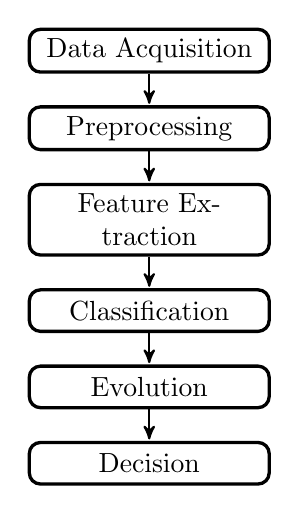
\begin{tikzpicture}
  [node distance=.4cm,
  start chain=going below,]
     \node[punktchain, join] (data) {Data Acquisition};\pause
     \node[punktchain, join] (Pre)  {Preprocessing};\pause
     \node[punktchain, join] (feature){Feature Extraction};\pause
     \node[punktchain, join] (cla) {Classification};\pause
     \node[punktchain, join, ] (evo) {Evolution};\pause
     \node[punktchain, join, ] (dec) {Decision};\pause

 \end{tikzpicture}

%%%%%%%%%%%%%%%%%%
\end{column}
\end{columns}

\end{frame}

\begin{frame}
\transboxout

\frametitle{PATTERN RECOGNITION MODEL}\pause
\begin{itemize}
\begin{columns}
\begin{column}{.7\textwidth}
 \item {\bf \underline{ Statistical model}:-} Pattern recognition system are based on statistics and probabilities. \pause
 \end{column}
 \begin{column}{.2\textwidth}
\begin{figure}
\includegraphics[width=\textwidth]{sta.jpg} \pause

\end{figure}
\end{column}
\end{columns}

 \begin{columns}
\begin{column}{.7\textwidth}
\item {\bf \underline{Syntactic model}:-} Structural models for pattern recognition and are based on the relation between features. Here the patterns are represented by structures.\pause

\end{column}
 \begin{column}{.2\textwidth}
\begin{figure}
\includegraphics[width=\textwidth]{syn.png}\pause

\end{figure}
\end{column}
\end{columns}

 \begin{columns}
\begin{column}{.7\textwidth}
\item {\bf \underline{ Template matching model}:-} In this model, a template or a prototype of the pattern to be recognized is available. \pause

\end{column}
 \begin{column}{.2\textwidth}
\begin{figure}
\includegraphics[width=\textwidth]{tem.jpg} \pause

\end{figure}
\end{column}
\end{columns}

 \begin{columns}
\begin{column}{.8\textwidth}
\item {\bf \underline{ Neural network model}:-} An artificial neural network (ANN) is a self-adaptive trainable process that is able to learn and resolve complex problems based on available knowledge.
\pause
\end{column}
 \begin{column}{.1\textwidth}
\begin{figure}
\includegraphics[width=\textwidth]{neu.png} \pause

\end{figure}
\end{column}
\end{columns}

\end{itemize}
\end{frame}

\begin{frame}
\transwipe

\frametitle{PATTERN CLASS}
\begin{itemize}

\begin{columns}
\begin{column}{.5\textwidth}
\item[$\#$]\onslide<2-> A Pattern class is a set of patterns sharing common attributes.%\pause
\item[$\#$]\onslide<4-> A collection of ``Similar" (not necessarily identical) objects.%\pause
\item[$\#$]\onslide<5-> During recognition given objects are assigned to prescribed classes.%\pause

\end{column}
 \begin{column}{.3\textwidth}
 \onslide<3->
\begin{figure}
\includegraphics[width=\textwidth]{cla.jpg}\pause

\end{figure}
\end{column}
\end{columns}
\end{itemize}

\begin{columns}

\begin{column}{.4\textwidth}
\begin{figure}
\onslide<6->
\includegraphics[width=\textwidth]{class.png}\pause
\onslide<6>
\caption{SR}
\end{figure}
\end{column}



\end{columns}
\end{frame}

\begin{frame}
\transsplitverticalout

\frametitle{CLASSIFICATION}\pause
\begin{itemize}
\item There are two main types of classification of pattern recognition.\pause
\end{itemize}
\begin{enumerate}
\item [$(1)$]{\bf \underline {Supervised Training / Learning}:-}Supervised learning is the machine learning task of learning a function that maps an input to an output based on example input-output pairs.\pause
\begin{figure}
\includegraphics[width=.5\textwidth]{sup.png}
\caption{Supervised Learning}\pause
\end{figure}
\end{enumerate}

\end{frame}

\begin{frame}
\transsplitverticalout

\frametitle{CLASSIFICATION}

\begin{enumerate}
\item[$(2)$] {\bf \underline {Unsupervised Training / Learning }:-}\pause Unsupervised learning is a branch of machine learning that learns from test data that has not been labeled, classified or categorized. Instead of responding to feedback, unsupervised learning identifies commonalities in the data and reacts based on the presence or absence of such commonalities in each new piece of data.\pause

\begin{figure}
\includegraphics[width=.5\textwidth]{uns.jpeg} \pause

\end{figure}
\end{enumerate}


\end{frame}

\begin{frame}
  % \transfade

\frametitle{APPLICATION OF PATTERN RECOGNITION}\pause
\framesubtitle{\underline{FINGERPRINT RECOGNITION}}\pause
 \begin{itemize}
 \item[Input] Fingerprint of some person.\pause
 \item[Output] The person identity.\pause
 \item[Uses] Useful in science such as computerized access control, criminal pursuit, etc...\pause
 \end{itemize}
 \begin{columns}
 \begin{column}{.65\textwidth}
\begin{figure}
\includegraphics[width=.65\textwidth]{fing.jpg}
\caption{Fingerprint}\pause
\end{figure} 
 \end{column}
 \begin{column}{.5\textwidth}
 %%%%%%%%%%%%%%%%%%%
 \begin{figure}
%
\href{run:fingure.mp4}{\includegraphics[width=.5\textwidth]{fin.jpg}} 
 
 %%%%%%%%%%%%%%%%%%%%
%\begin{figure}
%\includegraphics[width=.5\textwidth]{fin.jpg}
\caption{Click On Fig.Video}\pause
\end{figure} 
 \end{column}
\end{columns}
\end{frame}

\begin{frame}
%\transfade

\frametitle{APPLICATION OF PATTERN RECOGNITION}\pause
\framesubtitle{\underline{CHARACTER RECOGNITION }}\pause
 \begin{itemize}
 \item Character recognition is useful in banking, postal applications, automated mail sorting, automatic license plate recognition, optical character recognition.\pause
 \end{itemize}
 

\begin{figure}
\includegraphics[width=.8\textwidth]{ocr.jpg}
\caption{Example(Optical Character Recognition)}\pause
\end{figure} 
 
 
\end{frame}

\begin{frame}
%\transfade

\frametitle{APPLICATION OF PATTERN RECOGNITION}\pause
\framesubtitle{\underline{SPEECH RECOGNITION }}\pause

\begin{itemize}
 \item[Input] Acoustic signal (Sound wave etc).\pause
 \item[Output] Contents of the speech.\pause
 \item[Uses] Useful in scenarios such as speech-to-text (STT), voice command and control (VCC), etc...\pause
 \end{itemize}
 \begin{columns}
 \begin{column}{.5\textwidth}
 \begin{figure}
 %%%%%%%%%%%%%%%%%%%%
 %
\href{run:voice.mp4}{\includegraphics[width=1\textwidth]{spee.png}} 
 
 %%%%%%%%%%%%%%%%%%%%%
%\begin{figure}
%\includegraphics[width=1\textwidth]{spee.png}
\caption{Click On Fig. To Know More}
\end{figure} 
 \end{column}
 
\end{columns}
\end{frame}

\begin{frame}
%\transfade

\frametitle{APPLICATION OF PATTERN RECOGNITION}\pause
\framesubtitle{\underline{FACE RECOGNITION}}\pause
 \begin{itemize}
 \item[Input] Image with several people.\pause
 \item[Output] Location of the peoples' face in image.\pause

 \end{itemize}
 \begin{columns}
 \begin{column}{.6\textwidth}
\begin{figure}
\includegraphics[width=.6\textwidth]{fface.jpg}
\caption{Face Detection}\pause
\end{figure} 
 \end{column}
 \begin{column}{.6\textwidth}
\begin{figure}
\includegraphics[width=.6\textwidth]{facef.jpg}
\caption{Age And Gender Detection}\pause
\end{figure} 
 \end{column}
\end{columns}
\end{frame}

\begin{frame}
%\transfade

\frametitle{APPLICATION OF PATTERN RECOGNITION}\pause
\framesubtitle{\underline{COMPUTER AIDED DIAGNOSIS }}\pause
 \begin{itemize}
 \item Computer Aided Diagnosis is useful in scenarios such as diagnosis of diseases and paramedical industry.\pause
 \end{itemize}
 

\begin{figure}
\includegraphics[width=.8\textwidth]{cad.jpg}\pause
%\caption{Example()}
\end{figure} 
 
 
\end{frame}

\begin{frame}
%\transfade

\frametitle{APPLICATION OF PATTERN RECOGNITION}\pause
\framesubtitle{\underline{SIGNATURE RECOGNITION}}\pause
 \begin{itemize}
 \item[Input] Signature of some person(Sequence of dots).\pause
 \item[Output] The signatory's identity.\pause
\item[Uses] Useful in scenarios such as digital signature verification, credit card anti-fraud, etc.\pause
 \end{itemize}
 \begin{columns}
 \begin{column}{.6\textwidth}
\begin{figure}
\includegraphics[width=.6\textwidth]{sig.jpg}
\caption{Signature}\pause
\end{figure} 
 \end{column}
 \begin{column}{.6\textwidth}
\begin{figure}
\includegraphics[width=.6\textwidth]{sigg.jpg}
\caption{Signature Sample}\pause
\end{figure} 
 \end{column}
\end{columns}
\end{frame}

\begin{frame}
\transboxout

\frametitle{ONE CASE STUDY IN PATTERN RECOGNITION}
\framesubtitle{\underline{OPTICAL MUSIC  RECOGNITION}}\pause

\begin{itemize}
\item {\bf \underline{INTRODUCTION}:-} The paper presents a pattern recognition study aimed on music notation recognition.It presents a variety of methods applied in optical music recognition technology.\pause

\item {\bf \underline{DEFINITION}:-}Optical music recognition (OMR) or Music OCR is the application of optical character recognition to interpret sheet music or printed scores into editable or playable form. Once captured digitally, the music can be saved in commonly used file formats, e.g. MIDI (for playback) and MusicXML (for page layout).\pause
\end{itemize}

\end{frame}

\begin{frame}
 \transboxin


\begin{enumerate}
\item[$\diamond$] {\bf {Optical Music Recognition Architecture}}
\end{enumerate}
\begin{figure}
    \centering
    \includegraphics<1->[width=1\textwidth]{"architecture".jpg}
    \caption{Typical architecture of an OMR processing system}
    \label{fig:my_label}
\end{figure}
\pause
\end{frame}

\begin{frame}
\transboxout

\begin{enumerate}
\item[$\diamond$]{\textbf {Properties of the musical symbols}}\\ \pause
Music notation is a kind of alphabet,shaped by a general consensus of opinion,used to express ways of interpreting a musical passage.It is the visual manifestation of pitch,dynamics,time,and timbre.Symbols indicating the choice of tones,their duration,and the way they are performed are important.\pause
 \end{enumerate}
 \begin{columns}
 \begin{column}{.7\textwidth}
 \begin{figure}
     
     \includegraphics[width=.7\textwidth]{"Music notation".jpg}
     \caption{Music Notation}
    % \label{fig:my_label}
 \end{figure}
 \end{column}
 \pause
 \begin{column}{.5\textwidth}
 \begin{figure}
 %
\href{run:ms.mp4}{\includegraphics[width=.5\textwidth]{start.jpg}} 
\caption{Play Sample Video}
\end{figure}
\end{column} 
 \end{columns}
\end{frame}

\begin{frame}
\transboxin

%\begin{columns}
%\begin{column}{0.7\textwidth}
\begin{itemize}
\item[$\diamond$]{\textbf {Image Preprocessing}:-}\\ \pause
The music scores processed by the state-of-art algorithms are mostly written in a standard modern notation.Enhancement,binarization,noise removal,blurring,etc. are the most common techniques for preprocessing.\pause
\end{itemize}
\begin{columns}
\begin{column}{0.4\textwidth}
\begin{figure}
    \includegraphics[width=.4\textwidth]{"musical notations".jpg}
    \caption{Early and modern}\pause
    %\label{fig:my_label}
\end{figure}
\end{column}
\begin{column}{0.42\textwidth}
%%%%%%%%%%%%%%%%%%%%%%%%%%%%%
\begin{figure}
%
\href{run:riu.mp3}{\includegraphics[width=.42\textwidth]{"ipre".jpg}}


%%%%%%%%%%%%%%%%%%%%%%%%%%%%
%\begin{figure}
    %\includegraphics[width=.42\textwidth]{"ipre".jpg}
    \caption{Play Music Sample}\pause
    %\label{fig:my_label}
\end{figure}
\end{column}
\begin{column}{0.38\textwidth}
\begin{figure}
    \includegraphics[width=.38\textwidth]{"ipre2".jpg}
    \caption{Image Processing}\pause
    %\label{fig:my_label}
\end{figure}
\end{column}
\end{columns}

\end{frame}

\begin{frame}
\transboxout
\begin{itemize}
\item[$\diamond$]{\bf{Staff Line Detection and Removal}:-}\\ \pause
It is needed to isolate the music symbols for a more efficient and correct detection of each symbol in the score.Finding local maxima on the horizontal project of the black pixels of the image,scanning vertical lines,grouping of vertical columns,etc.are techniques used for detection.\pause
\end{itemize}

\begin{columns}
\begin{column}{0.5\textwidth}
\begin{figure}
    \includegraphics[width=.5\textwidth]{"staf".jpg}
    \caption{Staff Line D\& R graphical}\pause
    %\label{fig:my_label}
\end{figure}
\end{column}
\begin{column}{0.5\textwidth}
\begin{figure}
    \includegraphics[width=.7\textwidth]{"staff".jpg}
    \caption{Staff Line D\& R }\pause
    %\label{fig:my_label}
\end{figure}
\end{column}
\end{columns}
\end{frame}

\begin{frame}
\transboxout

\begin{itemize}
\item[$\diamond$]{\bf{Symbol Segmentation and Recognition}:-}\\ \pause
It consists of locating and isolating the musical objects to identify them.The most usual approach is a hierarchical decomposition of the music image.A music sheet is first analyzed and split by staffs and then the elementary graphic symbols are extracted.As a result,three hypothesis occur and then used to make a consistent decision.\pause
\end{itemize}
\begin{figure}
\includegraphics[width=.8\textwidth]{sym.png}
\caption{Symbols}\pause
\end{figure}
\end{frame}

\begin{frame}
\transboxin

\begin{itemize}
\item[$\diamond$]{\bf{Musical Notation Construction and Final Representation}:-}\pause
It is the final stage that extract the musical semantics from the graphically recognized shapes and store them in a musical data structure.\pause
\begin{figure}
    
    \includegraphics[width=.8\textwidth]{final stucture.jpg}
    \caption{Summary Of Optical Music Recognition}
    %\label{fig:my_label}
\end{figure}
\end{itemize}
\end{frame}


\begin{frame}
\transsplithorizontalin

\frametitle{ADVANTAGE OF PATTERN RECOGNITION}
\begin{itemize}
\item[$\star$] {\bf{\underline{Advantages}}:-}\\ \pause
\begin{itemize}
\item[$\ast$] Pattern recognition solves classification problems. \pause
\item[$\ast$] Pattern recognition solves the problem of fake bio metric detection.\pause
\item[$\ast$] It is useful for cloth pattern recognition for visually impaired blind people. \pause
\item[$\ast$] It helps in speaker diarization.\pause
\item[$\ast$] We can recognize particular object from different angle.\pause
\end{itemize}
\end{itemize}
\end{frame}

\begin{frame}
\transsplithorizontalout

\frametitle{DISADVANTAGE OF PATTERN RECOGNITION}
\begin{itemize}
\item[$\star$] {\bf{\underline{Disadvantages}}:-}\\ \pause
\begin{itemize}
\item[$\ast$] Syntactic pattern recognition approach is a complex to implement and it is very slow process.\pause
\item[$\ast$] Sometime to get better accuracy, larger dataset is required. \pause
\item[$\ast$] It cannot explain why a particular object is recognized.\pause
\begin{itemize}
\item[Example] My face {\bf \it Vs} my friend's face.\pause
\end{itemize}
\end{itemize}
\end{itemize}
\end{frame}


\begin{frame}
\transdissolve

\frametitle{CONCLUSION}
\begin{columns}
\begin{column}{.7\textwidth}
\begin{itemize}
\item[$\odot$]\onslide<3-> Structural methods concerned structure sense to encode but additional process to define primitives are required.%\pause
\item[$\odot$]\onslide<4-> Template matching is simple to implement but the template size must be small to decrease computational delay.%\pause
\item[$\odot$]\onslide<5-> Statistical methods highly dependent on the assumption of distribution.%\pause
\item[$\odot$]\onslide<6> Neural networks can adaptively refine the classifier and the decision surface in principle can be arbitrarily implemented.%\pause
\end{itemize}
\end{column}
\begin{column}{.6\textwidth}
\begin{figure}
\onslide<1->
\includegraphics[width=.5\textwidth]{conclusion.jpg}%\pause
\end{figure}
\end{column}
\end{columns}
\end{frame}


\begin{frame}

%\transfade
\frametitle{FUTURE WORKS}\pause
\begin{itemize}
\begin{columns}
\begin{column}{.4\textwidth}
\item[$\triangleright$] Frequency domain or wavelet domain.\pause
\end{column}
\begin{column}{.5\textwidth}
\includegraphics[width=.5\textwidth]{freq.jpg}\pause
\end{column}
\end{columns}
\begin{columns}
\begin{column}{.4\textwidth}
\item[$\triangleright$] Image compression method to face recognition.\pause
\end{column}
\begin{column}{.5\textwidth}
\includegraphics[width=.5\textwidth]{compression.jpg}\pause
\end{column}
\end{columns}
\begin{columns}
\begin{column}{.4\textwidth}
\item[$\triangleright$] Video-based face recognition.\pause
\end{column}
\begin{column}{.5\textwidth}
\includegraphics[width=.5\textwidth]{videoface.png}\pause
\end{column}
\end{columns}
\begin{columns}
\begin{column}{.4\textwidth}
\item[$\triangleright$] Adding color factor into face recognition.\pause
\end{column}


\begin{column}{.5\textwidth}
\includegraphics[width=.5\textwidth]{colorface.jpg}\pause
\end{column}
\end{columns}
\end{itemize}
\end{frame}


\begin{frame}
\transwipe

\frametitle{REFERENCES}\pause
\begin{thebibliography}{}
\bibitem{}  Bishop, Christopher M. (2006). Pattern Recognition and Machine Learning . \pause
 \bibitem{}   Armando Vieira, Data Scientist at Closer(Address- \href{URL}{ https://www.sshare.net/armandovieira2/pattern-recognition-18230948})\pause
\bibitem{} REHMAT ULLAH,  Graphic Designer and SEO Expert and Maaz Hasan, Intern at Hewlett Packard India Pvt. Ltd Adderss- \href{URL}{https://www.ss.net/MaazHasan/pattern-recognition-37839488}\pause

\bibitem{} Azriel Rosenfeld$^1$, Harry Wechsler$^2$, Received 19 December 1999, revised 30 March 2000, Center for Automation Research, University of Maryland, College Park, MD 20742-3275,\url{Email: ar@cfar.umd.edu} Department of Computer Science, George Mason University, Fairfax, VA 22030-4444,\url{Email: wechsler@cs.gmu.edu} \pause

\end{thebibliography}
\end{frame}
{
%\usebackgroundtemplate{\includegraphics[width=1\textwidth]{thankyou.jpg}}
\begin{frame}
%\transuncover
\end{frame}

}
\end{document}


%%% Local Variables: 
%%% mode: latex
%%% TeX-master: t